% Shared vector grammar. Generated figure TeX files inline this source.
\documentclass[tikz,border=4mm,12pt]{standalone}
\usepackage[UTF8,fontset=fandol]{ctex}
\usepackage{amsmath,amssymb,bm}
\renewcommand{\familydefault}{\sfdefault}
\hyphenpenalty=10000
\exhyphenpenalty=10000
\usetikzlibrary{arrows.meta,backgrounds,calc}
\definecolor{Ink}{HTML}{273648}
\definecolor{Muted}{HTML}{607086}
\definecolor{Ctx}{HTML}{85898F}
\definecolor{Qst}{HTML}{4F8FA5}
\definecolor{Opt}{HTML}{5A9A6E}
\definecolor{Gen}{HTML}{B89A5E}
\definecolor{Hid}{HTML}{8A74B5}
\definecolor{Wgt}{HTML}{E0904F}
\definecolor{Lgt}{HTML}{C95B5B}
\definecolor{Idx}{HTML}{7E8B9B}
\definecolor{Msk}{HTML}{3F5A78}
\newcommand{\Unit}{0.30}
\newcommand{\Offset}{0.12}
\newcommand{\BinarySupport}{0}
\newcounter{texture}
\tikzset{
 flow/.style={-{Latex[length=2mm,width=1.5mm]},draw=Ink!75!Canvas,line width=.65pt},
 tensorlabel/.style={font=\small,text=Ink,align=center,inner sep=0pt},
 tenshape/.style={font=\scriptsize,text=Muted,align=center,inner sep=0pt},
 stage/.style={font=\small\bfseries,text=Muted,align=left,anchor=west},
 operation/.style={draw=Ink!25!Canvas,fill=Canvas,rounded corners=2pt,align=center,
  font=\small,text=Ink,inner sep=5pt,line width=.5pt},
}
% The last two axes define a matrix face. Leading axes use offset sheets.
% Every symbolic dimension maps to the same cell count throughout the set.
\newcommand{\Tensor}[9]{%
 \stepcounter{texture}
 \pgfmathsetmacro{\ww}{#5*\Unit}
 \pgfmathsetmacro{\hh}{#4*\Unit}
 \pgfmathsetmacro{\xx}{#2-\ww/2}
 \pgfmathsetmacro{\yy}{#3-\hh/2}
 \ifnum#7>0
  \foreach \s in {#7,...,1}{
   \path[draw=#6!40!Canvas,fill=Canvas,line width=.45pt,rounded corners=.7pt]
    ({\xx+\s*\Offset},{\yy+\s*\Offset}) rectangle ++(\ww,\hh);}
 \fi
 \foreach \r in {1,...,#4}{\foreach \c in {1,...,#5}{
  \ifnum\BinarySupport>0
   \pgfmathtruncatemacro{\level}{\BinarySupport==1?(\c>3-\r?75:0):(\BinarySupport==2?(\c<=4-\r?75:0):(\c<=\r?75:0))}
  \else
   \pgfmathtruncatemacro{\tone}{mod(\r*13+\c*7+\arabic{texture}*11,7)}
   \pgfmathtruncatemacro{\level}{\tone<3?30:(\tone<6?55:80)}
  \fi
  \path[fill=#6!\level!Canvas,rounded corners=.5pt]
   ({\xx+(\c-1)*\Unit+.021},{\yy+\hh-\r*\Unit+.021})
    rectangle ++({\Unit-.042},{\Unit-.042});}}
 \ifnum\BinarySupport>0
  \path[draw=Msk!35!Canvas,line width=.4pt] (\xx,\yy) rectangle ++(\ww,\hh);
 \fi
 \coordinate (#1-w) at (\xx,#3);
 \coordinate (#1-e) at ({\xx+\ww+#7*\Offset},#3);
 \node[tensorlabel] at (#2,{\yy-.28}) {$#8$};
 \node[tenshape] at (#2,{\yy-.63}) {$#9$};
}
% Exact binary support; row i is a query and column j a key.
\newcommand{\Support}[5]{%
 \foreach \i in {1,...,#4}{\foreach \j in {1,...,#4}{
  \pgfmathtruncatemacro{\on}{#5}
  \ifnum\on>0
   \path[fill=Msk!65!Canvas,rounded corners=.4pt]
    ({#2+(\j-1)*\Unit+.021},{#3-\i*\Unit+.021})
     rectangle ++({\Unit-.042},{\Unit-.042});
  \fi}}
 \path[draw=Ink!35!Canvas,line width=.4pt] (#2,#3) rectangle ++({#4*\Unit},{-#4*\Unit});
}
\newcommand{\Meaning}[7]{%
 \node[anchor=north west,fill=Ink!4!Canvas,rounded corners=3pt,inner sep=9pt,
  text width=#3cm-18pt,align=left,font=\small] (meaning) at (#1,#2) {
  \begin{tabular}{@{}p{1.8cm}@{\hspace{7pt}}p{\dimexpr #3cm-2.8cm\relax}@{}}
   \textbf{#4} & \raggedright #5\tabularnewline[6pt]
   \textbf{#6} & \raggedright #7\tabularnewline
  \end{tabular}};
}

\definecolor{Canvas}{HTML}{18212C}
\definecolor{Ink}{HTML}{E2EAF3}
\definecolor{Muted}{HTML}{AABCD0}
\definecolor{Ctx}{HTML}{ABB3BE}
\definecolor{Qst}{HTML}{72B8D0}
\definecolor{Opt}{HTML}{83C396}
\definecolor{Gen}{HTML}{D9BC7B}
\definecolor{Hid}{HTML}{B49BDB}
\definecolor{Wgt}{HTML}{F0AB71}
\definecolor{Lgt}{HTML}{ED9191}
\definecolor{Idx}{HTML}{A9BBD1}
\definecolor{Msk}{HTML}{91B6DF}
\pagecolor{Canvas}

\begin{document}
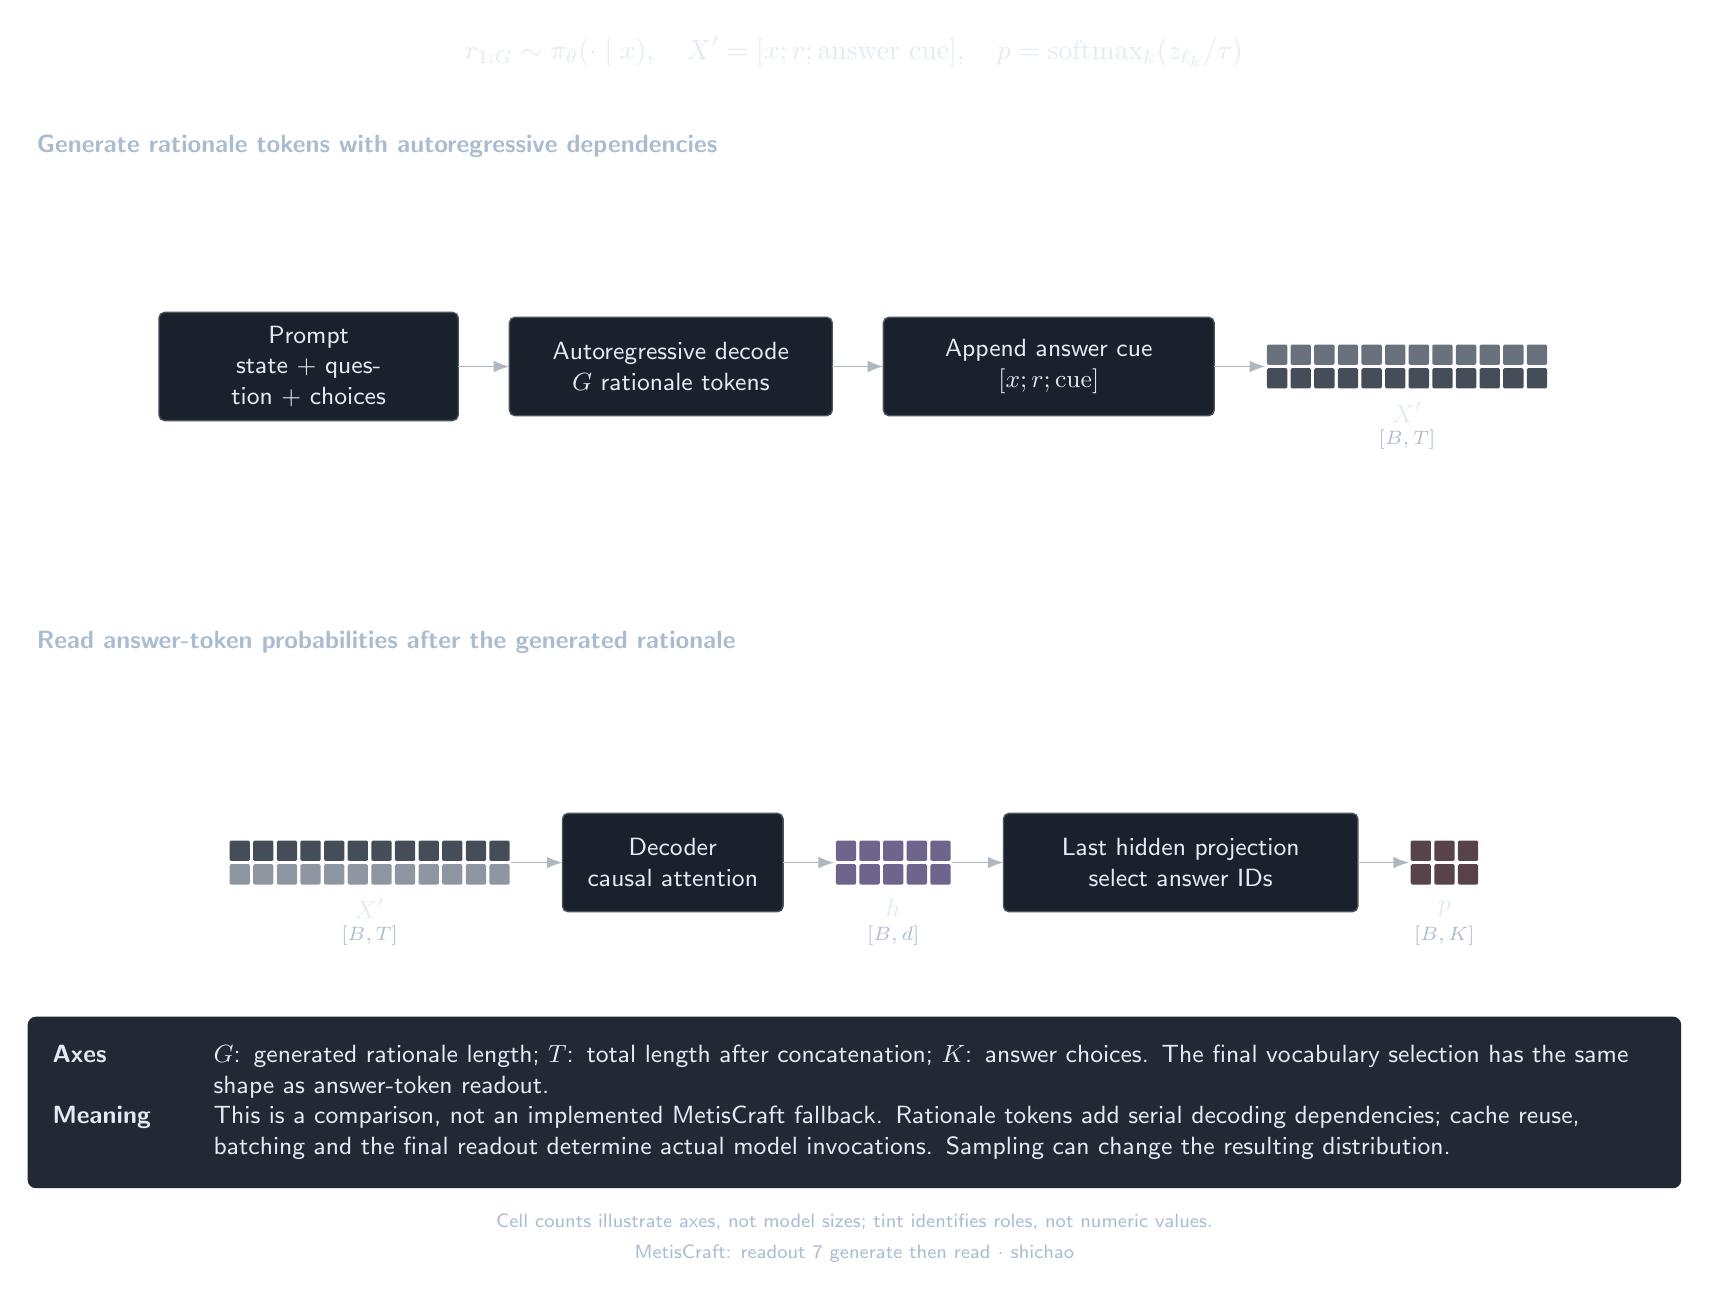
\begin{tikzpicture}[x=1cm,y=1cm,text=Ink]
\node[font=\normalsize,align=center] at (10.500,4.0) {$\displaystyle r_{1:G}\sim\pi_\theta(\cdot\mid x),\quad X'=[x;r;\mathrm{answer\ cue}],\quad p=\operatorname{softmax}_k(z_{\ell_k}/\tau)$};
\node[stage] at (0,2.800) {Generate rationale tokens with autoregressive dependencies};
\node[operation,minimum width=3.800cm,minimum height=1.250cm,text width=3.450cm] (r0n0) at (3.575,-0.000) {Prompt\\state + question + choices};
\coordinate (r0n0-w) at (1.675,-0.000);\coordinate (r0n0-e) at (5.475,-0.000);
\node[operation,minimum width=4.100cm,minimum height=1.250cm,text width=3.750cm] (r0n1) at (8.175,-0.000) {Autoregressive decode\\$G$ rationale tokens};
\coordinate (r0n1-w) at (6.125,-0.000);\coordinate (r0n1-e) at (10.225,-0.000);
\draw[flow] (r0n0-e) -- (r0n1-w);
\node[operation,minimum width=4.200cm,minimum height=1.250cm,text width=3.850cm] (r0n2) at (12.975,-0.000) {Append answer cue\\$[x;r;\mathrm{cue}]$};
\coordinate (r0n2-w) at (10.875,-0.000);\coordinate (r0n2-e) at (15.075,-0.000);
\draw[flow] (r0n1-e) -- (r0n2-w);
\renewcommand{\BinarySupport}{0}
\Tensor{r0n3}{17.525}{-0.000}{2}{12}{Ctx}{0}{X'}{[B,T]}
\draw[flow] (r0n2-e) -- (r0n3-w);
\node[stage] at (0,-3.500) {Read answer-token probabilities after the generated rationale};
\renewcommand{\BinarySupport}{0}
\Tensor{r1n0}{4.350}{-6.300}{2}{12}{Ctx}{0}{X'}{[B,T]}
\node[operation,minimum width=2.800cm,minimum height=1.250cm,text width=2.450cm] (r1n1) at (8.200,-6.300) {Decoder\\causal attention};
\coordinate (r1n1-w) at (6.800,-6.300);\coordinate (r1n1-e) at (9.600,-6.300);
\draw[flow] (r1n0-e) -- (r1n1-w);
\renewcommand{\BinarySupport}{0}
\Tensor{r1n2}{11.000}{-6.300}{2}{5}{Hid}{0}{h}{[B,d]}
\draw[flow] (r1n1-e) -- (r1n2-w);
\node[operation,minimum width=4.500cm,minimum height=1.250cm,text width=4.150cm] (r1n3) at (14.650,-6.300) {Last hidden projection\\select answer IDs};
\coordinate (r1n3-w) at (12.400,-6.300);\coordinate (r1n3-e) at (16.900,-6.300);
\draw[flow] (r1n2-e) -- (r1n3-w);
\renewcommand{\BinarySupport}{0}
\Tensor{r1n4}{18.000}{-6.300}{2}{3}{Lgt}{0}{p}{[B,K]}
\draw[flow] (r1n3-e) -- (r1n4-w);
\Meaning{0}{-8.250}{21.000}{Axes}{$G$: generated rationale length; $T$: total length after concatenation; $K$: answer choices. The final vocabulary selection has the same shape as answer-token readout.}{Meaning}{This is a comparison, not an implemented MetisCraft fallback. Rationale tokens add serial decoding dependencies; cache reuse, batching and the final readout determine actual model invocations. Sampling can change the resulting distribution.}
\node[font=\scriptsize,text=Muted,anchor=north,align=center] at ($(meaning.south)+(0,-.2)$) {Cell counts illustrate axes, not model sizes; tint identifies roles, not numeric values.\\[3pt]MetisCraft: readout 7 generate then read $\cdot$ shichao};
\end{tikzpicture}
\end{document}
